\subsection{Divisão e conquista}

    Divisão e Conquista é uma estratégia para projeto de algoritmos utilizada 
    pela primeira vez por Anatolii Karatsuba em 1960. Esta técnica consiste em dividir um problema maior 
    recursivamente em problemas menores, até que o problema possa ser resolvido diretamente. Por fim, a
    solução do problema inicial é dada através da combinação dos resultados de todos os problemas 
    menores computados. Exemplos de problemas conhecidos que usam desta estratégia, é o problema de 
    ordenação interna(usando quicksort ou mergesort), ou o problema dos pares de pontos próximos.

\subsubsection{Pares de pontos próximos}

    Dado um conjunto de n pontos em um espaço, é preciso encontrar os dois pontos do conjunto que possuem a 
    menor distância um do outro. Este problema possui mais de uma possível implementação, porém 
    uma das mais eficientes é utilizando divisão e conquista.

    \begin{figure}[ht]
        \centering
        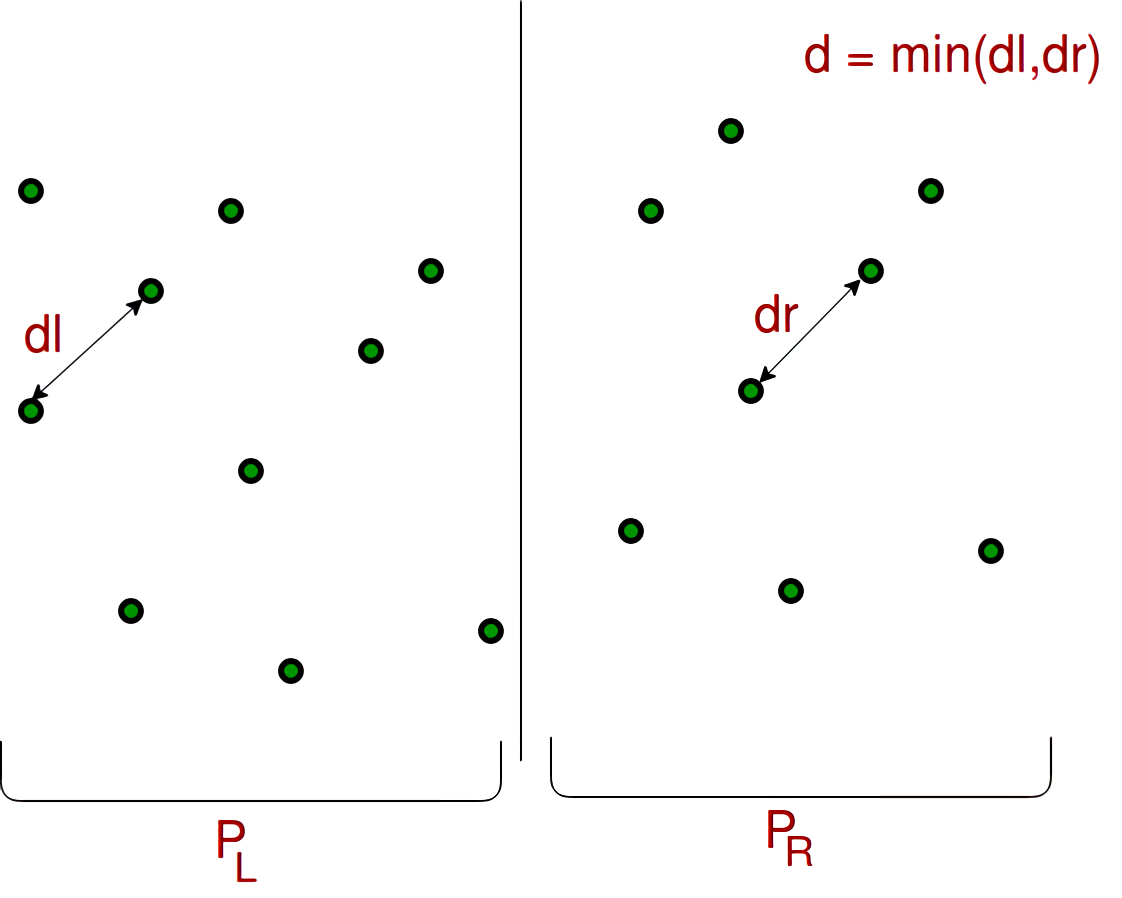
\includegraphics[width=.5\textwidth]{divide-and-conquer.png}
        \caption{Uma representação visual da separação dos pontos}
        \label{fig:divide-and-conquer}
    \end{figure}

    Supondo que a entrada para o problema é um conjunto de pontos com o eixo x já ordenado,
    encontramos o ponto do meio, separamos o conjunto ao meio, e então recursivamente descobrimos
    as menores distâncias entre os conjuntos separados, para então achar a solução geral.

    \begin{algorithm}
        \caption{Closest pair of points} 
        \begin{algorithmic}[1]
        \Procedure{Divide-and-conquer}{}
        \State {$\text{colors} \gets \text{[G.vertex]}$}
        \For{$\text{v in G.V}$}
        \If{$\text{colors[v] == WHITE}$}
        \State {$\textbf{visit(v,colors)}$}
        \EndIf
        \EndFor
        \EndProcedure
        \end{algorithmic}
      \end{algorithm}

      \subsubsection{Divisão e Conquista Vs Backtracking}

      \begin{itemize}
          \item Devido a maneira como ambos são conceptualizados, ambos 
          possuem a natureza de serem recursivos.
          \item Devido a natureza da estratégia de backtracking, tais algoritmos costumam ter 
          implementações recursivas, enquanto que algoritmos gulosos tentam 
          buscar a melhor escolha local de forma iterativa.
      \end{itemize}

      \subsubsection{Divisão e Conquista Vs Branch and Bound}

      \begin{itemize}
          \item Enquanto divisão e conquista divide a entrada do usuário(Ex: divide o vetor de números para 
          ordená-los), para resolver os sub-problemas e então resolver a combinação desses problemas. A outra estratégia, 
          divide o espaço da solução para o problema.
          \item Devido a natureza da estratégia de backtracking, tais algoritmos costumam ter 
          implementações recursivas, enquanto que algoritmos gulosos tentam 
          buscar a melhor escolha local de forma iterativa.
      \end{itemize}

\newpage